%=======================================================================
%  Findings
%=======================================================================
\section{Findings}
\label{sec:findings}

This section reports what the five experiments produced, organised by
finding rather than by experiment. Each subsection states the finding,
gives the evidence, and says what it rests on.
\tabref{tab:findings-summary} summarises the six.

Findings F1--F4 answer the core research objectives: model the three
attacks, implement countermeasures, and demonstrate experimentally
whether the countermeasures reduce attack success. F5 and F6 go beyond
those objectives. Having established that the countermeasures work, the
threshold analysis asks the inverse question --- how much countermeasure
is actually \emph{required} --- and the coalition analysis asks whether
evaluating vectors one at a time understates the achievable attack.
Both are extensions to the original scope rather than part of it, and
they are reported as such.

\begin{table}[htbp]
\centering
\caption{Summary of findings.}
\label{tab:findings-summary}
\small
\begin{tabular}{@{}p{0.5cm}p{6.6cm}p{6.0cm}@{}}
\toprule
\textbf{\#} & \textbf{Finding} & \textbf{Principal evidence} \\
\midrule
F1 & Detection is a sharper lever than budget; success collapses over a
narrow band of $q$ rather than declining smoothly &
E1 budget and detection sweeps; \figref{fig:detection} \\
\addlinespace
F2 & Monte Carlo reproduces the exact value to $\sim$$10^{-4}$; the
Chernoff bound never failed but is loose by \BriberyChernoffGap{} &
E1 triangulation; \figref{fig:twosided} \\
\addlinespace
F3 & Countermeasures cut success probability by
\SybilRelReduction--\BriberyRelReduction\%, but residual risk
concentrates in identity verification &
E1; \tabref{tab:headline}, \figref{fig:comparison} \\
\addlinespace
F4 & Chain integrity and election correctness are independent: the
ledger was never violated and elections were stolen anyway &
E2; \figref{fig:flip} \\
\addlinespace
F5 & Attacks stop paying at detection far below what full protection
delivers: deterrence is roughly \ProtectionHeadroom$\times$ cheaper
than prevention &
E4; \tabref{tab:thresholds}, \figref{fig:critical} \\
\addlinespace
F6 & Combining vectors beats the best single vector in
\CoalitionBetterCount{} of \CoalitionScenarioCount{} scenarios, where
two of three are individually infeasible &
E5; \tabref{tab:coalition}, \figref{fig:coalition} \\
\bottomrule
\end{tabular}
\end{table}

\subsection{Overview}

\tabref{tab:headline} gives the headline comparison across the
\TotalTrials{} matched pairs per vector. All three vectors fall sharply
under the protected configuration, and every bootstrap confidence
interval on the paired reduction excludes zero comfortably.

\begin{table}[htbp]
\centering
\caption{Headline experimental results across 2{,}500 paired randomised trials per vector.}
\label{tab:headline}
\small
\resizebox{\textwidth}{!}{%
\begin{tabular}{lrrrrccr}
\toprule
Attack & Baseline & Protected & Absolute red. & Relative red. (\%) & 95\% CI & MC error & Bound holds (\%) \\
\midrule
Bribery & 0.350 & 0.064 & 0.287 & 81.859 & [0.269, 0.304] & 8.0e-05 & 100.000 \\
Sybil & 0.480 & 0.136 & 0.345 & 71.779 & [0.327, 0.362] & 4.0e-04 & 100.000 \\
Ballot Stuffing & 0.442 & 0.116 & 0.325 & 73.695 & [0.308, 0.343] & 3.9e-04 & 100.000 \\
\bottomrule
\end{tabular}%
}
\vspace{2pt}
{\footnotesize\textit{Note.} Confidence intervals are bootstrap intervals on the mean paired reduction (10{,}000 resamples). ``Bound holds'' is the percentage of trials with a mathematically valid Chernoff region in which the bound was not violated.}
\end{table}


\subsubsection*{Which probability is being reported}
\label{sec:findings-measures}

Two of the three vectors pass fraudulent votes through \emph{two}
independent gates, so they admit two different success probabilities,
and the distinction has to be made explicit before any table is read.

\begin{itemize}\setlength{\itemsep}{2pt}
\item $P(\text{accepted} \geq m)$ --- the probability that at least $m$
fraudulent votes clear the \emph{acceptance} gate (Sybil registration,
or ballot admission). This is an intermediate quantity: it ignores
detection entirely, is always the larger of the two, and is not
comparable across vectors.
\item $P(\text{surviving} \geq m)$ --- the probability that at least
$m$ fraudulent votes clear \emph{both} gates, being accepted
\emph{and} escaping detection. This is the headline measure. Every
figure, every stated finding and every conclusion in this chapter uses
it.
\end{itemize}

Bribery has a single effective gate, because detection is already
folded into its per-attempt success probability $1-q$; for bribery the
two measures coincide. For Sybil and ballot stuffing they do not, and
the gap is substantial --- under the baseline configuration the Sybil
acceptance-only figure is \SybilAcceptedBaseline{} against a
both-gates figure of \SybilBaseline{}, and the corresponding
ballot-stuffing pair is \BallotStuffingAcceptedBaseline{} against
\BallotStuffingBaseline{}.

Both quantities are reported, because the difference between them is
itself a result: it isolates how much of the countermeasure effect
comes from tightening registration and admission rather than from
detection. The per-vector tables therefore carry an explicit
\code{measure} column, and the aggregate tables report the headline
measure only, so that the numbers a reader is most likely to quote are
the same in every table. A test asserts this agreement
(\code{tests/test\_reporting\_consistency.py}), because the two
measures were at one point reported side by side without being named,
which made correct numbers look inconsistent.


\begin{finding}
\finhead{F3 --- effect of countermeasures (RQ3)}
Across \TotalTrials{} matched pairs, the protected configuration
reduced mean attack success probability from \BriberyBaseline{} to
\BriberyProtected{} for bribery (\BriberyRelReduction\% relative), from
\SybilBaseline{} to \SybilProtected{} for Sybil attacks
(\SybilRelReduction\%), and from \BallotStuffingBaseline{} to
\BallotStuffingProtected{} for ballot stuffing
(\BallotStuffingRelReduction\%). The 95\% bootstrap interval for the
bribery reduction is $[\BriberyCILow, \BriberyCIHigh]$.
\end{finding}

One feature of the distributions is worth stating before the detail,
because it governs how the means should be read. The per-trial success
probabilities are strongly bimodal: the baseline bribery distribution
has a mean of \BriberyBaseline{} but a median of
\BriberyBaselineMedian{} and a standard deviation of
\BriberyBaselineStd. Most scenarios are either comfortably safe or
comfortably lost. A mean of \BriberyBaseline{} therefore does not
describe a typical election facing a 35\% risk; it describes a
population in which roughly a third of elections are in serious
trouble and the rest are not. This is why the analysis reports
thresholds (F5) rather than resting on averages.

\subsection{F1 --- Budget and detection are not symmetric levers}
\label{sec:findings-levers}

Bucketing the \TotalTrials{} trials by attacker budget shows success
probability rising steadily with budget under both configurations. The
baseline curve crosses even odds inside the sampled range; the
protected curve never does, at any budget tested.

The budget effect is gradual and saturating: additional money buys
additional attempts only until the capacity ceiling
$T = \min(N, \lfloor B/R \rfloor)$ binds, after which it buys nothing.
There are two distinct infeasibility regimes: below the $T = m$
contour the attacker cannot reach the threshold even with a perfect
success rate, and above the $T = N$ contour the electorate is
exhausted, so further budget buys nothing at all.

The detection effect has a different shape entirely.
\figref{fig:detection} holds every other parameter fixed and sweeps
only $q$: success stays near certainty until the survival probability
$1 - q$ falls far enough that the mean drops below the threshold, at
which point it collapses over a narrow band. Detection does not erode
an attack; past a point, it ends it.

\begin{figure}[H]
\centering
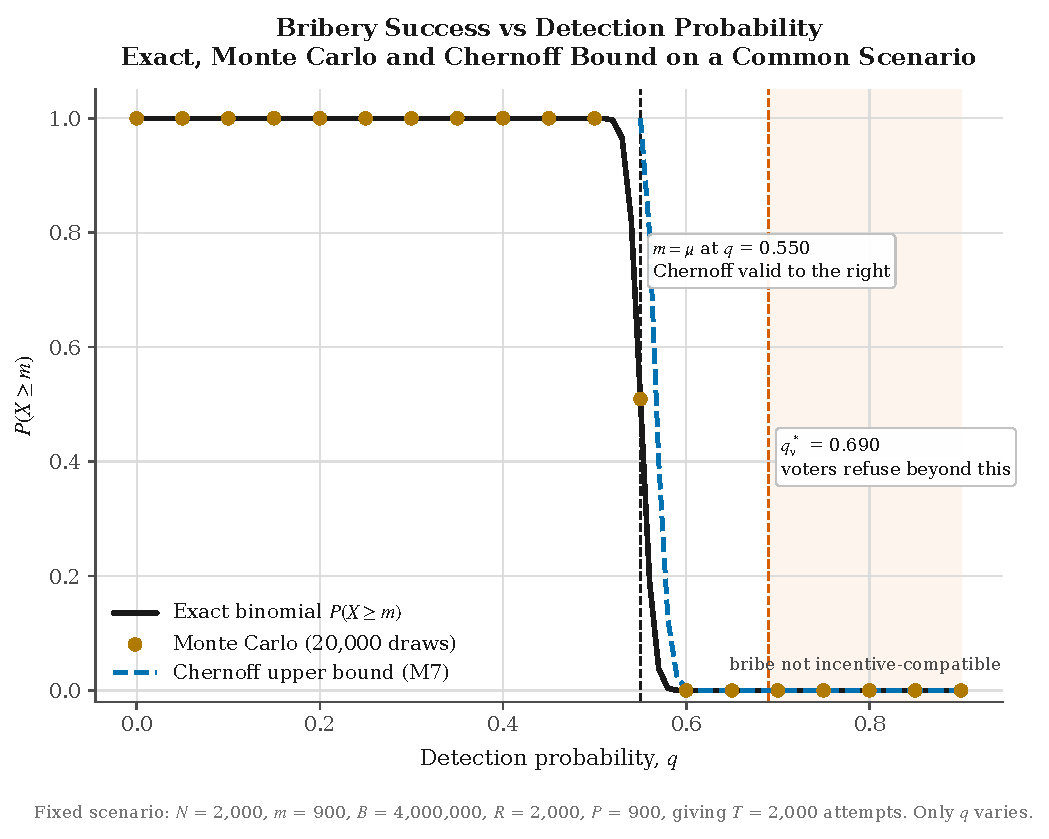
\includegraphics[width=0.86\textwidth]{fig_01_method_comparison.pdf}
\caption[Exact, Monte Carlo and Chernoff comparison]{Exact binomial,
Monte Carlo and Chernoff bound against detection probability on one
fixed scenario. Averaging these three quantities across heterogeneous
randomised trials would compare them on different sub-populations ---
the bound exists only where $m > \mu$ --- so this figure varies only
$q$.}
\label{fig:detection}
\end{figure}

Two mechanisms produce that collapse and they compound. The mean
surviving count $T(1-q)$ falls linearly in $q$, and the binomial
concentrates tightly around its mean, so once the mean crosses the
threshold the tail probability falls away exponentially. On top of
that, bribery carries the rational-voter gate: beyond
$q_v^* = R/(R+P)$ the bribe is refused outright.
\figref{fig:utility} shows that surface, with the closed-form threshold
traced over the numerically computed zero contour. Both are evaluated
by the production modules --- the surface by the M1 implementation, the
curve by the T2 solver --- so their coinciding checks that the solver
returns the root of the utility function as coded. It is a check on the
implementation, not independent evidence for the model: T2 is the
analytic root of M1, so agreement is expected, and only a coding error
could separate the two.

\begin{figure}[H]
\centering
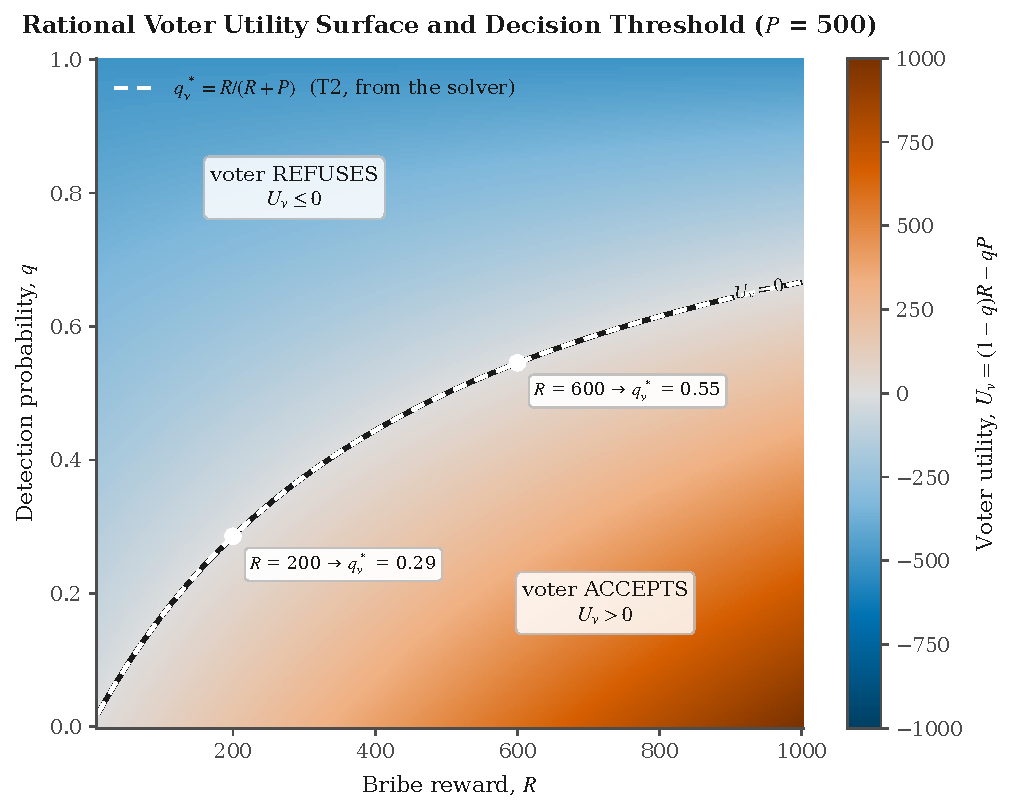
\includegraphics[width=0.78\textwidth]{fig_02_voter_utility_threshold.pdf}
\caption[Voter utility surface and decision threshold]{Rational voter
utility $\Uv = (1-q)R - qP$, with the $\Uv = 0$ decision boundary and
the closed-form indifference threshold $q_v^{*} = R/(R+P)$ drawn
together.}
\label{fig:utility}
\end{figure}

\begin{finding}
\finhead{F1 --- where defensive effort pays (RQ1)}
Budget and detection are not interchangeable. Budget raises success
gradually and saturates at a capacity ceiling that no further spending
moves. Detection produces a sharp collapse, because it lowers the mean
and --- for bribery --- eventually removes the attacker's supply of
willing voters altogether. A defender choosing between raising the cost
of an attack and raising the chance of catching it should prefer the
latter.
\end{finding}

\subsection{F2 --- The three methods agree, and each has a distinct use}
\label{sec:findings-methods}

RQ2 asks how well the Monte Carlo estimate and the Chernoff bound
reproduce the exact value.

The Monte Carlo estimator is accurate: mean absolute error against the
exact binomial probability was \BriberyMCError{} for bribery,
\SybilMCError{} for Sybil and \BallotStuffingMCError{} for ballot
stuffing, with worst-case errors of \BriberyMCMaxError{},
\SybilMCMaxError{} and \BallotStuffingMCMaxError{} respectively.
A convergence sweep over sample sizes from \ConvergenceMinSize{} to
\ConvergenceMaxSize{} draws (\code{results/csv/monte\_carlo\_convergence.csv})
shows the estimator settling to within \ConvergenceTolerance{} of the
exact value from \ConvergenceSettles{} draws onward, reaching an
absolute error of \ConvergenceFinalError{} at the largest sample size.
The \MonteCarloTrials{} draws used per scenario therefore sit inside the
converged regime. A two-standard-error envelope is the looser test here
and is reported in the same file: since it is a 95\% interval, isolated
excursions are expected and two of the nine sample sizes show one, which
is why the settling point is quoted against a fixed tolerance rather
than against the envelope.

The Chernoff bound held in every trial where it was mathematically
defined: \BriberyChernoffHolds\% of \BriberyChernoffValid{} valid
bribery trials, \SybilChernoffHolds\% of \SybilChernoffValid{} Sybil
trials and \BallotStuffingChernoffHolds\% of
\BallotStuffingChernoffValid{} ballot-stuffing trials, with no
violation anywhere. It is also loose --- a mean gap of
\BriberyChernoffGap{} for bribery --- which is the expected behaviour
of a bound rather than a defect.

The bound is one-sided, however, and it exists only where the threshold
sits above the mean. That left the scenarios with $m \leq \mu$ --- the
ones in which the attack is \emph{most} likely to succeed --- with no
analytic statement at all. The two-sided certificate of
Section~\ref{sec:certificate} closes that gap by applying the
$(1-\delta)$ lower-tail form to the failure event, and
\figref{fig:twosided} validates both directions against the exact value
on the same experiment.

\begin{figure}[H]
\centering
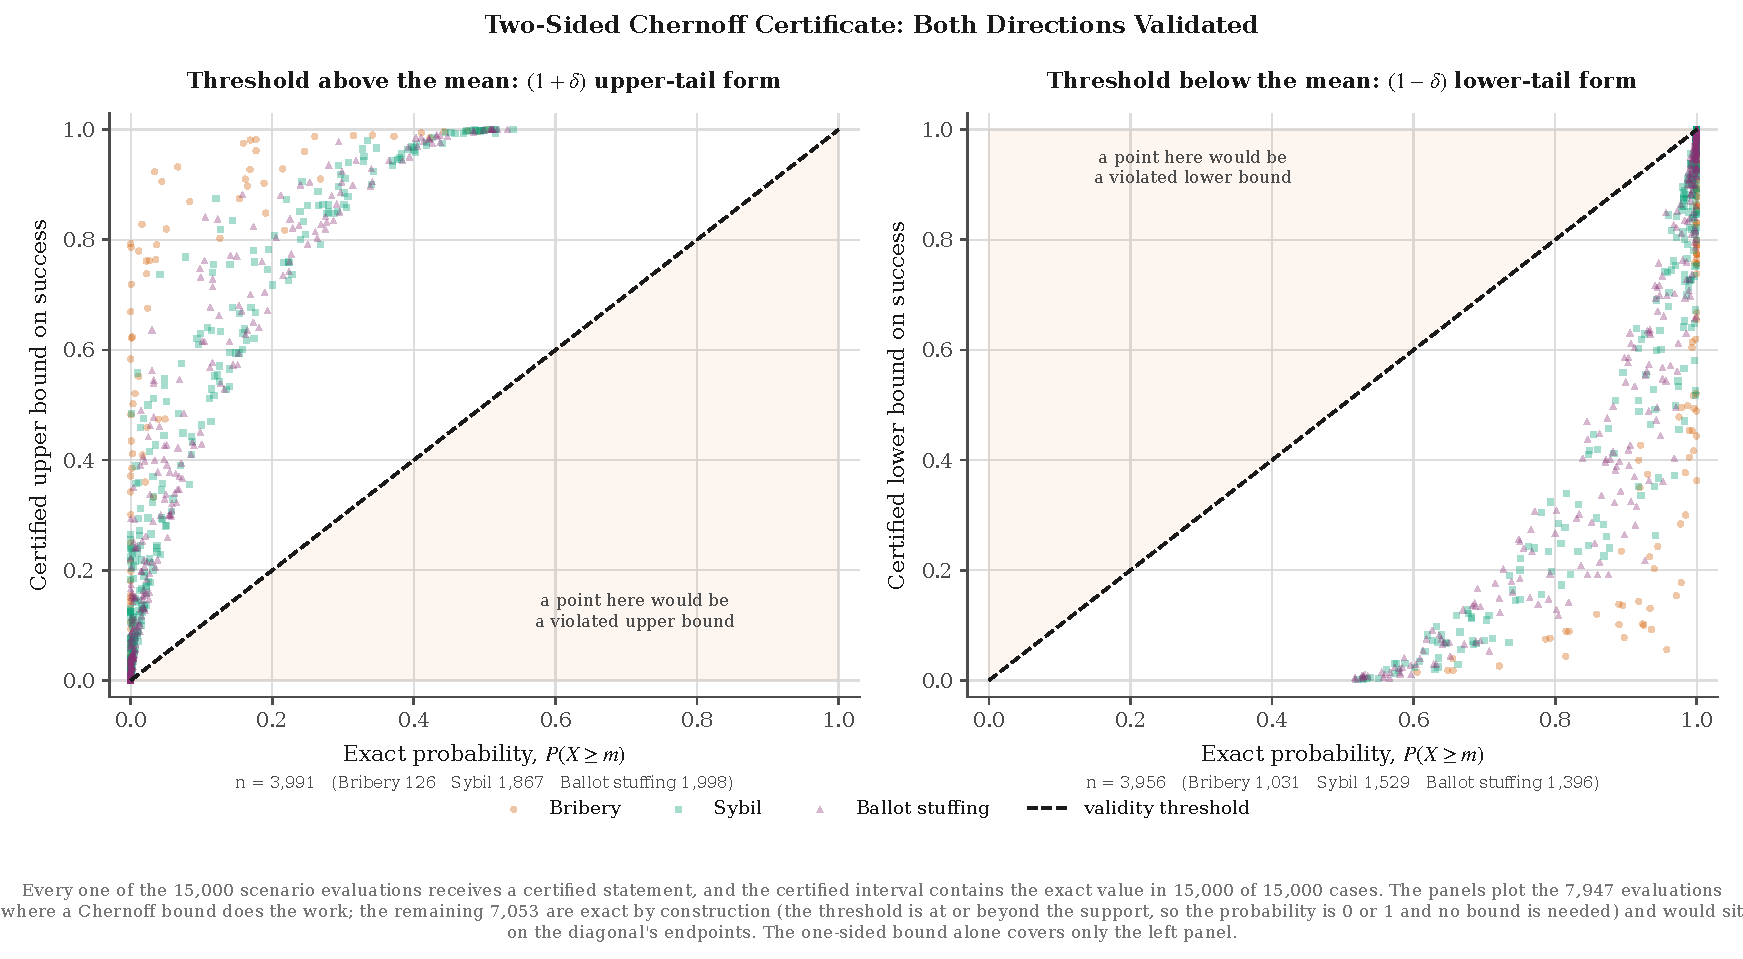
\includegraphics[width=\textwidth]{fig_03_chernoff_two_sided.pdf}
\caption[Two-sided Chernoff certificate]{Both Chernoff directions
validated. Left: threshold above the mean, where the $(1+\delta)$
upper-tail form certifies success from above --- valid points lie on or
above the diagonal. Right: threshold below the mean, where the
$(1-\delta)$ lower-tail form applied to the failure event certifies
success from below --- valid points lie on or below it. No point falls
on the wrong side of either diagonal.}
\label{fig:twosided}
\end{figure}

With the certificate in place, every one of the 15{,}000 scenario
evaluations carries a guaranteed statement, and the certified interval
contains the exact value in 100\% of them.

\begin{finding}
\finhead{F2 --- when to use which method (RQ2)}
Use the exact binomial value whenever it is affordable; it always was
here, even at $N = \SThreeN$. Use Monte Carlo where the quantity has no
closed form --- the concrete election simulation, for instance. Use the
Chernoff bound when a \emph{provable} statement is required rather than
an estimate: it is the only one of the three that certifies a margin as
safe independently of how the simulation ran, which is what makes the
certified margin $m_{\varepsilon}$ meaningful as a security claim
rather than an observation.
\end{finding}

\subsection{F3 --- Countermeasures work, but not uniformly}

Both remaining vectors behave more smoothly than bribery, because
neither has a consent gate: a forged identity does not decline. Their
success probability rises steadily with effort rather than switching
off at a threshold.

Sybil attacks are the most resilient of the three under the tested
parameter distribution, retaining a mean success probability of
\SybilProtected{} under protection --- roughly twice the protected
bribery figure of \BriberyProtected. The reason is structural rather
than numerical: bribery is suppressed twice over, once by detection and
once by the voter's refusal, whereas a Sybil attack is suppressed only
by detection. \figref{fig:comparison} shows the three vectors together.

\begin{figure}[H]
\centering
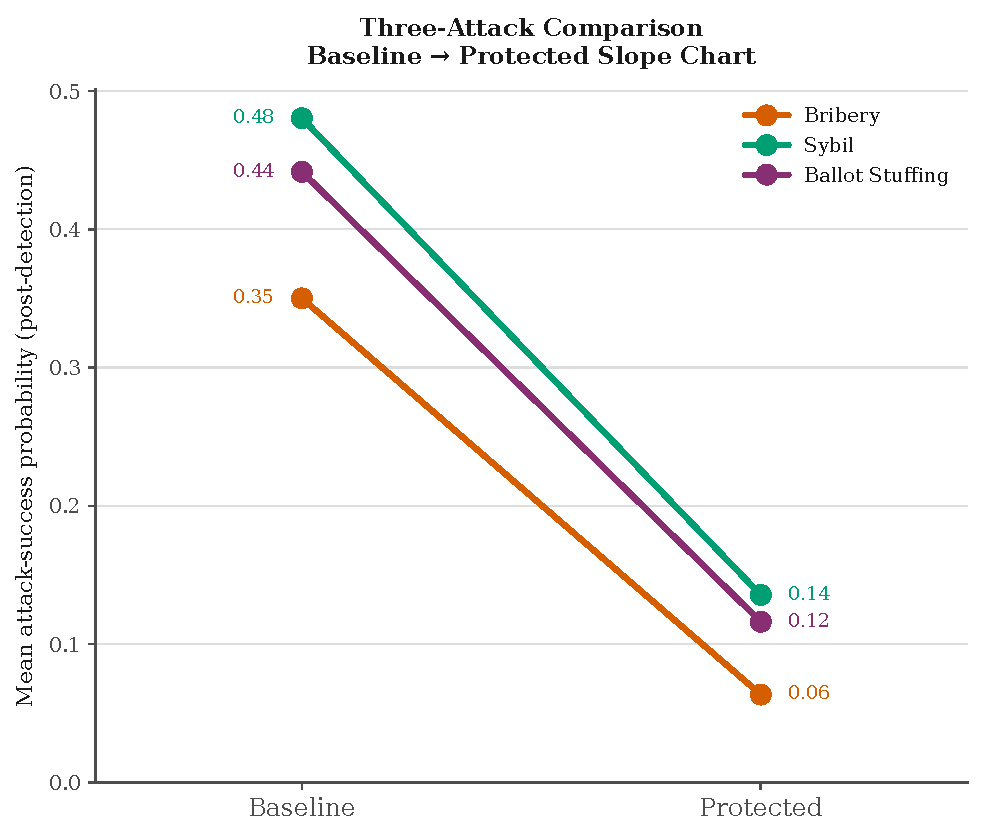
\includegraphics[width=0.64\textwidth]{fig_04_attack_comparison.pdf}
\caption[Three-attack comparison]{Mean success probability for the
three vectors, baseline against protected.}
\label{fig:comparison}
\end{figure}

The distributions add something the means conceal: under protection
they are compressed toward zero rather than merely shifted downward.
The countermeasures remove the upper tail of highly successful attacks,
which is the part of the distribution that actually decides elections.
They do not remove the attack. Under protection the Sybil and
ballot-stuffing vectors retain mean success probabilities of
\SybilProtected{} and \BallotStuffingProtected{} respectively, so the
defensible claim is that attack success is \emph{substantially reduced}
under the modelled countermeasures, not that it is eliminated.

\begin{finding}
\finhead{F3b --- where the residual risk sits}
Identity verification, not vote recording, is the binding constraint.
Sybil attacks remain the most successful vector under protection
(\SybilProtected{} mean success probability) because the ledger's
integrity guarantees say nothing about whether the identity behind a
ballot is real. This is consistent with voter authentication being
repeatedly flagged as an open problem in the systematic
reviews~\cite{ohize2025,rahul2025}. A deployment that hardens the chain
while leaving registration weak has hardened the wrong layer.
\end{finding}

\subsection{F4 --- Chain integrity and election correctness are independent}
\label{sec:findings-concrete}

The results so far are probabilities. \figref{fig:flip} reports what
happened when \ElectionTrials{} elections were genuinely mined on a
proof-of-work chain, attacked, and re-tallied from the chain to see who
actually won.

\begin{figure}[H]
\centering
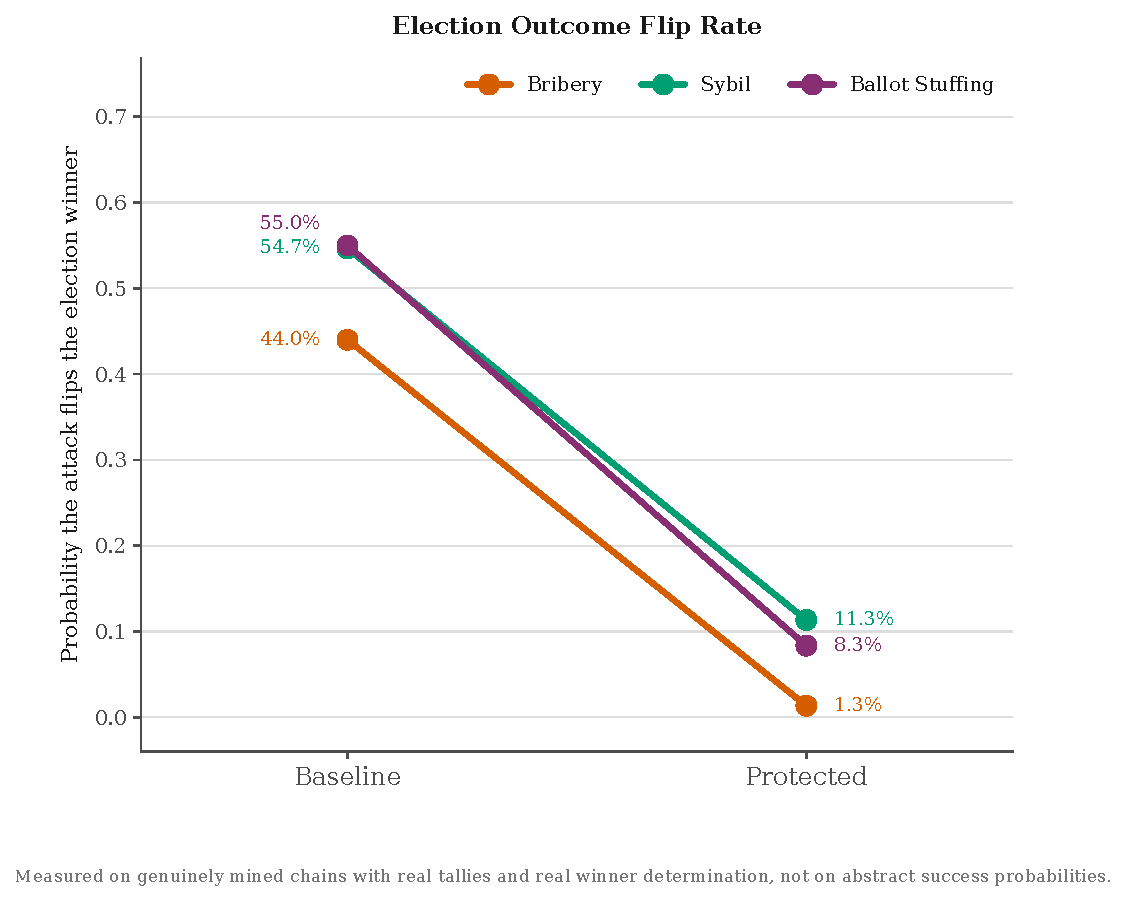
\includegraphics[width=0.64\textwidth]{fig_05_election_flip_rate.pdf}
\caption[Election outcome flip rate]{Probability that an attack flips
the winner of a concrete, blockchain-recorded election.}
\label{fig:flip}
\end{figure}

Baseline flip rates were \FlipBriberyBaseline\% for bribery,
\FlipSybilBaseline\% for Sybil and \FlipBallotStuffingBaseline\% for
ballot stuffing, falling under protection to \FlipBriberyProtected\%,
\FlipSybilProtected\% and \FlipBallotStuffingProtected\%. This is the
cross-layer check that Section~\ref{sec:method-twolayer} exists to
provide: two independent implementations --- one analytic, one a mined
chain --- agree in magnitude, in the direction and size of the
protection effect, and in placing bribery lowest in both layers. They
do not agree on the ordering of the top two: the analytic layer puts
Sybil (\SybilBaseline{}) above ballot stuffing (\BallotStuffingBaseline{}),
while the concrete layer reverses them, at \FlipSybilBaseline\% against
\FlipBallotStuffingBaseline\%. That gap is a third of a percentage point
on \ElectionTrials{} trials per vector --- well inside sampling error ---
so the two vectors are better read as indistinguishable at the concrete
layer than as ranked.

Individual trials make this concrete. For a representative flipped
baseline election, the attacker's surviving fraudulent votes carry the
target past the opponent's tally, while the protected run on the
\emph{same} starting election leaves the original winner in place.

\begin{finding}
\finhead{F4 --- the central observation}
Chain integrity was \ChainIntegrityHeld{} in any of the
\ElectionTrials{} trials. In the \FlipBriberyBaseline\% of baseline
bribery trials that flipped the winner, the blockchain was working
perfectly: every fraudulent vote was correctly formed, correctly mined
and permanently recorded, and the validity check passed afterwards.
Immutability guarantees that a wrong result cannot subsequently be
altered. It does not guarantee that the result is right. This is the
quantitative form of the argument Park et al.~\cite{park2021} make
qualitatively.
\end{finding}

\subsection{F5 --- Deterrence is far cheaper than prevention}
\label{sec:thresholds-results}

\tabref{tab:thresholds} collects every threshold for the five benchmark
scenarios. The critical detection probability $q_d^{*}$ --- the point at
which mounting the attack stops paying --- lies between
\CriticalDetectionMin{} and \CriticalDetectionMax{} across the
\CriticalDetectionBindingCount{} scenarios where detection is the
binding constraint. The protected configuration operates at
$q = \ProtectedQ$, roughly \ProtectionHeadroom{} times higher than the
strongest of those requirements.

\begin{table}[htbp]
\centering
\caption{Critical thresholds for the five benchmark scenarios under the baseline configuration.}
\label{tab:thresholds}
\small
\resizebox{\textwidth}{!}{%
\begin{tabular}{lrrrrrrrrrrr}
\toprule
Scenario & $N$ & $m$ & $R^*$ & $q_v^*$ & $T_{\min}$ & $q_d^*$ & $B^*$ & $T^*$ & $m_\alpha$ & $m_\varepsilon$ & $P(X \geq m)$ \\
\midrule
S1 & 100 & 35 & 52 & 0.118 & 38 & 0.118 & 2,880 & 37 & 34 & --- & 0.423 \\
S2 & 10,000 & 1,943 & 68 & 0.118 & 2,089 & 0.072 & 249,480 & 2,083 & 1,937 & --- & 0.328 \\
S3 & 100,000 & 19,015 & 63 & 0.111 & 20,016 & 0.050 & 2,998,650 & 20,000 & 19,000 & 19,515 & 0.320 \\
S4 & 5,000 & 4,758 & 26 & 0.167 & 5,008 & 0.051 & 499,400 & 5,000 & 4,750 & --- & 0.316 \\
S5 & 5,000 & 550 & 26 & 0.167 & 579 & 0.000 & 57,100 & 0 & 76 & --- & 0.000 \\
\bottomrule
\end{tabular}%
}
\vspace{2pt}
{\footnotesize\textit{Note.} $R^*$ minimum bribe a rational voter accepts (T1); $q_v^*$ voter-indifference detection (T2); $T_{\min}$ attempts for even odds (T3); $q_d^*$ critical detection at which attacking stops paying (T5); $B^*$ break-even budget (T4); $T^*$ utility-maximising attempts; $m_\alpha$ margin beaten at even odds (T7); $m_\varepsilon$ Chernoff-certified safe margin at $\varepsilon = 10^{-3}$ (T6). A dash means the threshold does not exist in the searched domain.}
\end{table}


\begin{figure}[H]
\centering
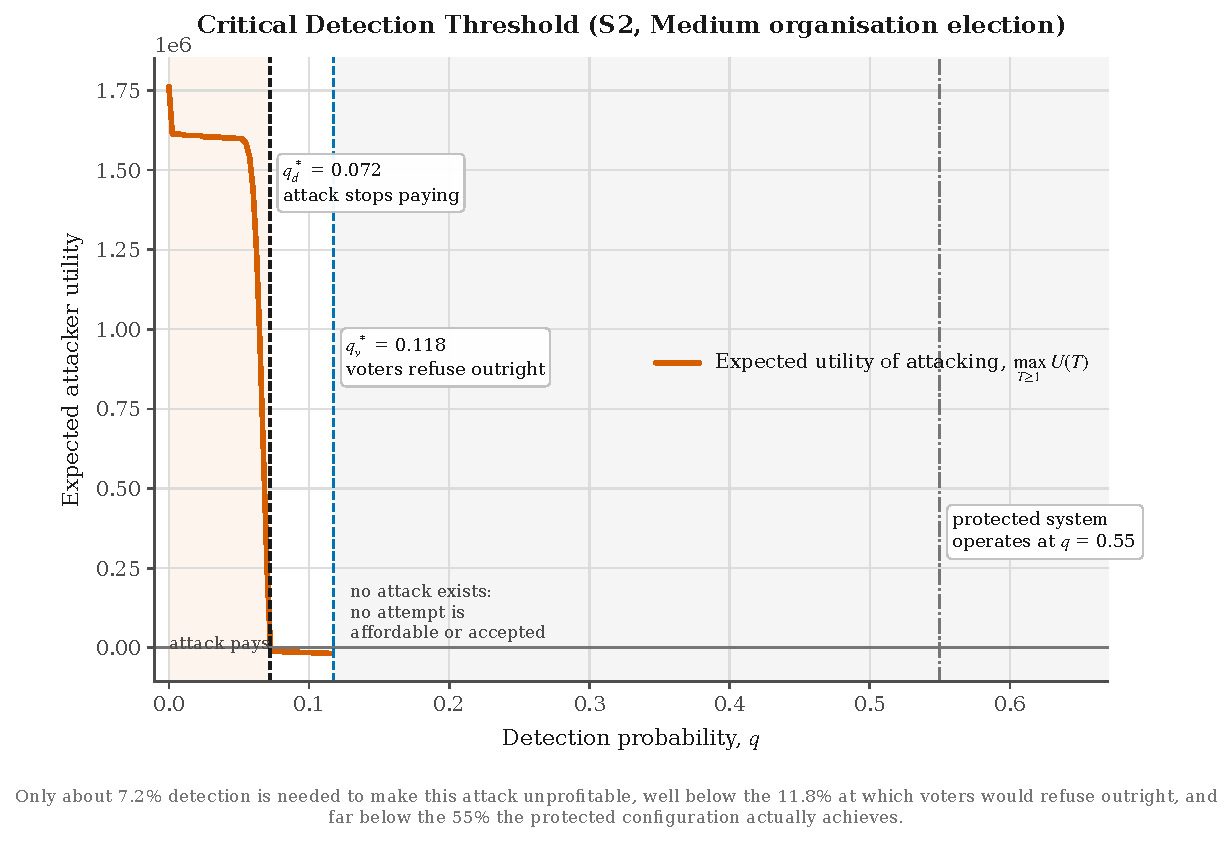
\includegraphics[width=0.80\textwidth]{fig_06_critical_detection.pdf}
\caption[Critical detection threshold]{Expected utility of attacking as
detection rises, for the medium-organisation scenario. Two thresholds
are marked: $q_d^{*}$, where the attack stops paying, and $q_v^{*}$,
where voters refuse outright.}
\label{fig:critical}
\end{figure}

The gap between the two thresholds is worth dwelling on. At $q_d^{*}$
the attack is still perfectly possible --- voters would accept, the
budget suffices --- but a rational attacker declines because the
expected return has gone negative. At $q_v^{*}$ the attack becomes
impossible, because the voters themselves refuse. Deterrence arrives
first and costs less; prevention arrives later and costs more.
\tabref{tab:thresholds} places all five scenarios against both
thresholds; every one of them sits far to the left of the protected
configuration's operating point.

\begin{finding}
\finhead{F5 --- minimum viable defence (RQ4)}
Making bribery unprofitable requires a detection probability of only
\STwoQCritical{} in the medium-organisation scenario and
\SThreeQCritical{} at national scale --- roughly one caught bribe in
fourteen, and one in twenty. This is far below the \ProtectedQ{} the
modelled countermeasures deliver. The security-relevant conclusion is
not that the countermeasures work, but that \emph{much weaker ones
would have}: the expensive part of the defence is buying certainty
rather than deterrence.
\end{finding}

\subsubsection{Break-even budget}

The break-even budget answers the complementary question: how much
would the attacker need before the attempt is worth making?
Sweeping budget for the medium-organisation scenario gives
$B^{*} = \STwoBStar$ against a scenario budget of \STwoBudget. Under the protected configuration the
curve never crosses zero at any budget, because the bribe is not
incentive-compatible at all.

\subsubsection{The contested band of margins}

\tabref{tab:thresholds} gives, for each scenario, the margin the
attacker beats at even odds ($m_\alpha$), the margin actually defended
($m$), and the margin the Chernoff bound certifies as safe
($m_\varepsilon$).

In four of the five scenarios the defended threshold sits inside its
band or a little above the attacker-reachable margin; the exception is
the low-budget scenario S5, where the defended margin exceeds
$m_\alpha$ by a factor of about seven and the attack is out of reach by
a wide margin rather than a narrow one. A certified margin
$m_\varepsilon$ exists for the national-scale scenario only --- in the
others the bound cannot certify even $m = n$ at
$\varepsilon = 10^{-3}$, which the solver reports rather than
silently omitting. At national scale the attacker reaches
\SThreeMReachable{} votes at even odds while the bound certifies safety
only from \SThreeMCertified{} --- a contested band roughly 500 votes
wide, with the defended threshold \SThreeM{} sitting just inside its
lower edge. That is the practical cost of the
bound's conservatism: within that band it declines to certify margins
that are in fact comfortably safe, and only exact computation resolves
them. \figref{fig:pmf} draws the same three thresholds on a single
distribution.

\begin{figure}[H]
\centering
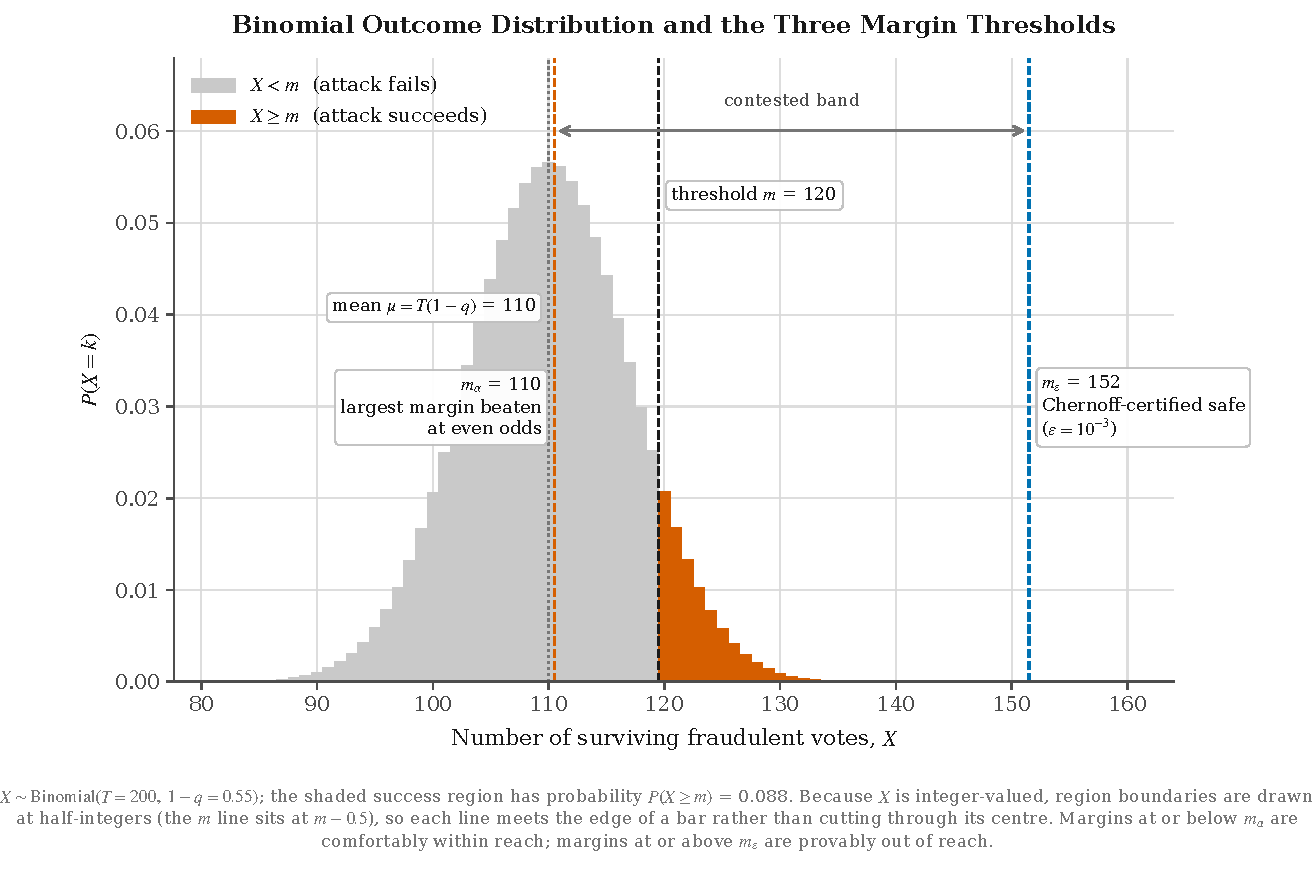
\includegraphics[width=0.86\textwidth]{fig_07_binomial_thresholds.pdf}
\caption[Binomial distribution with margin thresholds]{The binomial
outcome distribution with its mean, the manipulation threshold, the
attacker-reachable margin and the Chernoff-certified safe margin all
marked.}
\label{fig:pmf}
\end{figure}

\subsubsection{The rational attacker does not spend everything}

\figref{fig:optimal} shows expected utility and flip probability
against the number of bribery attempts. Utility is single-peaked: it
rises while further bribes still move the flip probability, then
declines once that probability saturates and each additional bribe buys
only cost and detection risk.

\begin{figure}[H]
\centering
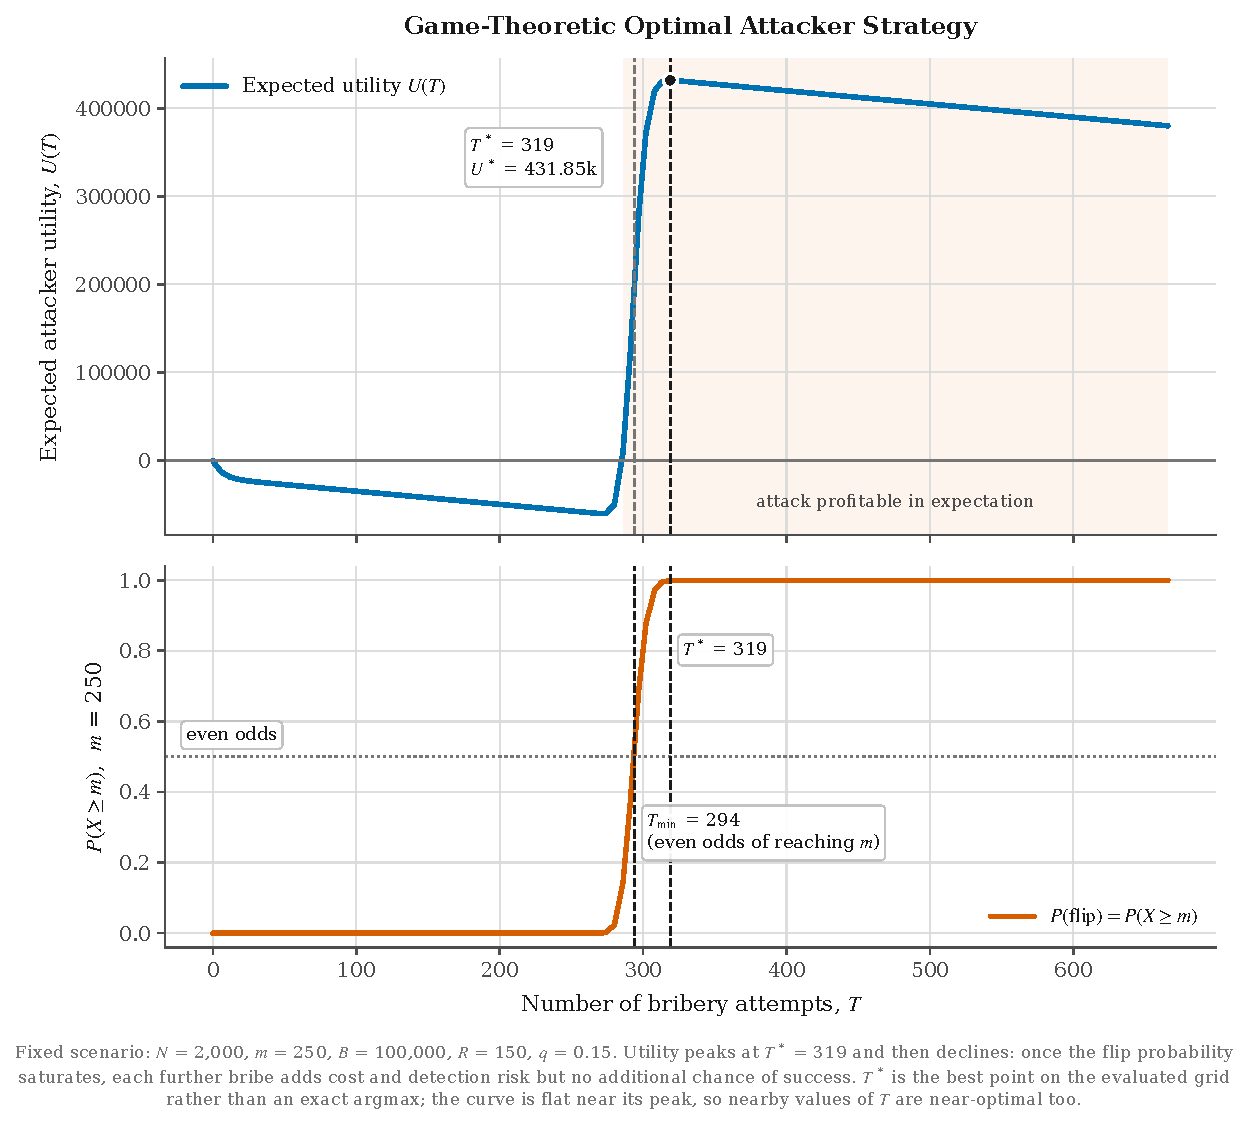
\includegraphics[width=0.80\textwidth]{fig_08_optimal_attacker.pdf}
\caption[Optimal attacker strategy]{Expected attacker utility (top) and
flip probability (bottom) against bribery attempts, with the
utility-maximising $T^{*}$ and the even-odds effort threshold
$T_{\min}$ marked.}
\label{fig:optimal}
\end{figure}

This matters for how the model is read. A budget-exhausting attacker
--- the implicit adversary of many security analyses --- does strictly
worse than a rational one, so optimising a defence against maximum
spending optimises against the wrong opponent. The observation is the
e-voting analogue of the selfish-mining result~\cite{eyal2014}: what an
attacker \emph{would choose} to do, not what they are capable of doing,
is the security-relevant quantity.

\subsection{F6 --- Combining vectors defeats what no single vector can}
\label{sec:coalition}

\subsubsection{No single vector suffices}

Once each vector is held to a realistic capacity ceiling --- forged
registrations limited to \SybilCeilingPct\% of the electorate by the
registration window, injected ballots to \BallotCeilingPct\% by the
turnout anomaly they would otherwise create, in the sense that election
forensics makes detectable~\cite{klimek2012} --- something striking
emerges from \tabref{tab:capacity}. Neither Sybil registration nor
ballot stuffing has an \emph{expected} yield that reaches the
manipulation threshold in any scenario.

The distinction matters and was sharpened after review. The capacity
ratio is $\Ex[X]/m$ --- a mean, not a ceiling. A ratio below one means
the attack falls short \emph{on average}; success is still possible on
an upward fluctuation. What makes the finding hold is how fast that
possibility decays: at S1's bribery ratio of 0.97 the exact success
probability is still \SOneBriberyPFull{}, at S3's ballot-stuffing ratio
of 0.99 it is \SThreeBallotPFull{}, and by a ratio of 0.74 it is
numerically zero. So the accurate statement is that Sybil registration
is effectively out of the running in every scenario, ballot stuffing
retains a small residual chance in the two largest ones, and no single
vector is a reliable route to the threshold --- not that any of them is
arithmetically impossible.

\begin{table}[htbp]
\centering
\caption{Capacity of each vector at full effort, as a multiple of the manipulation threshold $m$ (baseline configuration).}
\label{tab:capacity}
\small
\resizebox{\textwidth}{!}{%
\begin{tabular}{lrrrr}
\toprule
Scenario & Bribery & Sybil & Ballot Stuffing & Combined \\
\midrule
S1 & 0.97 & 0.41 & 0.54 & 1.92 \\
S2 & 1.00 & 0.74 & 0.97 & 2.71 \\
S3 & 1.00 & 0.76 & 0.99 & 2.75 \\
S4 & 1.00 & 0.15 & 0.20 & 1.35 \\
S5 & 0.14 & 0.26 & 0.61 & 1.01 \\
\bottomrule
\end{tabular}%
}
\vspace{2pt}
{\footnotesize\textit{Note.} Values are EXPECTED surviving votes over the threshold, so a value below 1.00 means the mean falls short --- not that the threshold is unreachable. Success remains possible on an upward fluctuation, though its probability collapses quickly: at a ratio of 0.97 the exact $P(X \geq m)$ is still 0.42 for bribery in S1, while by a ratio of 0.74 it is numerically zero. Every entry here falls below 1.00; the budget-feasible optimal coalition clears it in four of the five scenarios (\tabref{tab:coalition}).}
\end{table}


\begin{figure}[H]
\centering
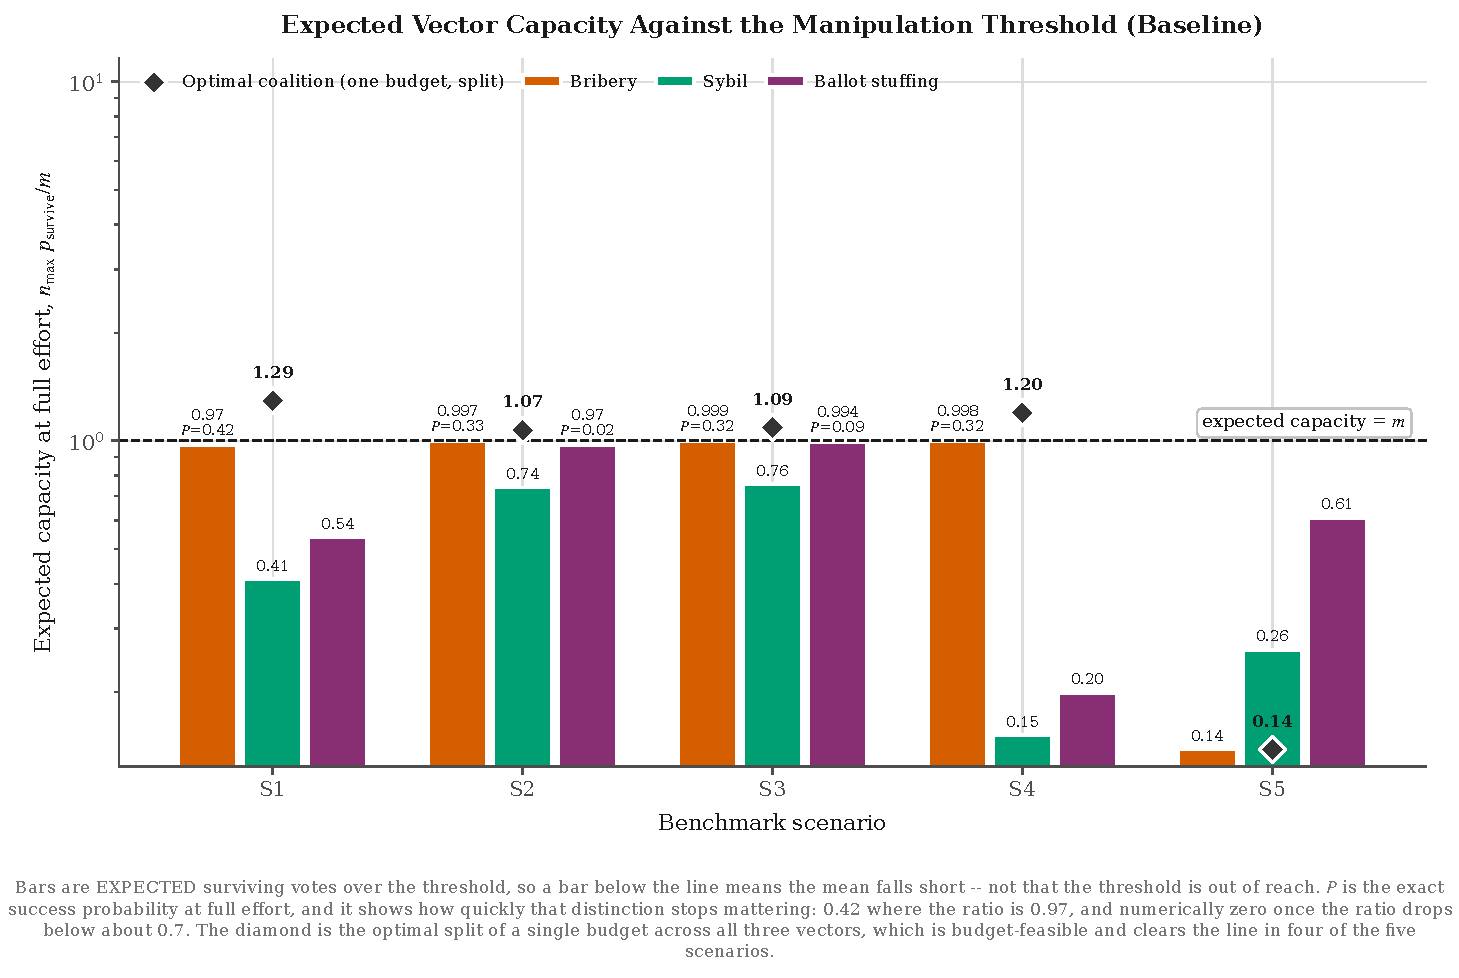
\includegraphics[width=0.86\textwidth]{fig_09_vector_capacity.pdf}
\caption[Vector capacity against the threshold]{\emph{Expected}
capacity of each vector at full effort, as a multiple of the
manipulation threshold. A bar below the line means the mean falls
short, not that the threshold is unreachable --- the annotated $P$ is
the exact success probability at full effort. The diamond is the
optimal split of a single budget across all three vectors, which is
budget-feasible.}
\label{fig:capacity}
\end{figure}

Analysed one vector at a time, this reads as a reassuring result: no
single vector is a dependable route to the threshold, and two of the
three are hopeless. It is the wrong conclusion, and the reason it is
wrong is that the attacker is not obliged to choose.

\subsubsection{The mixed strategy}
\label{sec:findings-coalition}

The search evaluates every way of splitting a single budget across the
three vectors, at a 0.05 resolution over the budget simplex, whose
corners are exactly the pure single-vector strategies. The optimum
leaves the corners in four of the five scenarios: it is strictly
interior in S1 $(0.35, 0.25, 0.40)$ and sits on an edge --- two vectors
funded, one not --- in S2, S3 and S4. Only S5, where no allocation
succeeds at all, returns a corner. The gain therefore comes from mixing
\emph{at least} two vectors rather than from using all three.

\begin{table}[htbp]
\centering
\caption{Optimal multi-vector budget allocation per scenario (baseline configuration).}
\label{tab:coalition}
\small
\resizebox{\textwidth}{!}{%
\begin{tabular}{lrrrrrlrr}
\toprule
Scenario & Bribery & Sybil & Ballot & $\mu_{\mathrm{total}}$ & Coalition $P$ & Best pure & Pure $P$ & Gain \\
\midrule
S1 & 35\% & 25\% & 40\% & 45 & 0.999 & Bribery & 0.423 & 0.576 \\
S2 & 0\% & 5\% & 95\% & 2,077 & 1.000 & Bribery & 0.328 & 0.672 \\
S3 & 0\% & 5\% & 95\% & 20,700 & 1.000 & Bribery & 0.320 & 0.680 \\
S4 & 10\% & 0\% & 90\% & 5,695 & 1.000 & Bribery & 0.316 & 0.684 \\
S5 & 100\% & 0\% & 0\% & 76 & 0.000 & Bribery & 0.000 & 0.000 \\
\bottomrule
\end{tabular}%
}
\vspace{2pt}
{\footnotesize\textit{Note.} Shares are the fractions of one budget allocated to each vector. Coalition success probability is computed exactly, by convolving the three binomial distributions rather than approximating their sum.}
\end{table}


\begin{figure}[H]
\centering
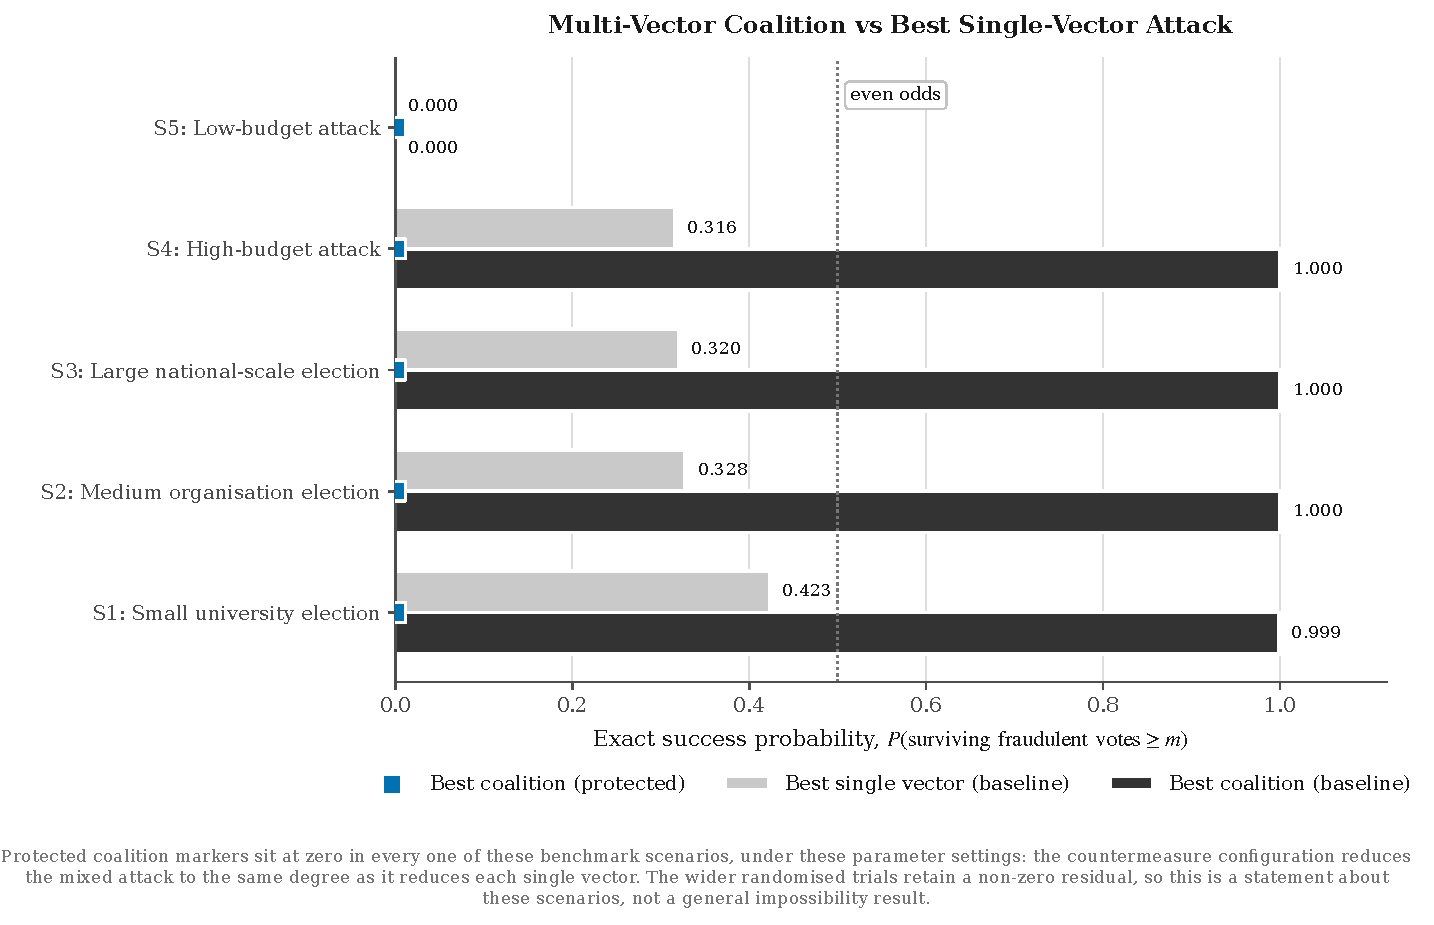
\includegraphics[width=0.88\textwidth]{fig_10_coalition_vs_pure.pdf}
\caption[Coalition against best single vector]{Best coalition attack
against best single-vector attack per scenario, with protected
coalition results overlaid.}
\label{fig:coalition}
\end{figure}

\begin{finding}
\finhead{F6 --- multi-vector attacks (RQ5)}
The optimal mixed strategy strictly outperforms the best single-vector
strategy in \CoalitionBetterCount{} of \CoalitionScenarioCount{}
baseline scenarios, raising mean success probability from
\BestPureMeanBaseline{} to \CoalitionMeanBaseline{}. In the high-budget
scenario, no single vector exceeds a success probability of
\SFourExactFlip{}, yet the mixture reaches near-certainty. A security
evaluation conducted one vector at a time therefore understates the
achievable attack --- not marginally, but qualitatively, by declaring
infeasible an attack that succeeds.
\end{finding}

The mechanism is capacity, not probability. Each vector saturates its
own ceiling long before the budget is exhausted, leaving money that
buys nothing more in that vector but a great deal in another.
Diversification here is not about hedging risk; it is about escaping a
binding constraint.

\subsubsection{Robustness of the coalition finding}

The coalition result depends on assumed relative costs and capacity
ceilings, none of which is empirically grounded.
The analysis therefore re-runs across \SensitivityConfigs{}
combinations of all four constants.

The coalition was at least as good as the best pure strategy in
\SensitivityAtLeastAsGood\% of configurations and strictly better in
\SensitivityStrictlyBetter\%. The qualitative conclusion does not
depend on the particular costs assumed --- as it should not, since a
mixed strategy can never be worse than the best pure one, the pure
strategies being corners of the same simplex. What the sweep
establishes is that the \emph{strict} improvement is not an artefact of
one convenient parameterisation.

\subsubsection{Countermeasures against the coalition}

Across the \CoalitionScenarioCount{} benchmark scenarios, the protected
configuration suppresses the coalition attack to the same degree as it
suppresses each vector alone: mean coalition success probability under
protection is \CoalitionMeanProtected{}. That figure is exactly zero
for these particular benchmark scenarios under these parameter
settings, and should be read as such rather than as a general claim
that the mixed attack is impossible --- the randomised trials, which
sample far more widely, leave a residual success probability of
\SybilProtected{} for Sybil attacks and \BallotStuffingProtected{} for
ballot stuffing. The bribery
gate closes in all \CoalitionScenarioCount{} scenarios, since
$\ProtectedQ > q_v^{*}$ everywhere, and the tightened acceptance and
detection probabilities pull the other two vectors' capacity below the
threshold. Coalition attacks are more dangerous than the single-vector
analysis suggests, but they are not differently defended.

\subsection{Scale effects}

One further result bears on deployment, and it is not uniform across
the vectors. Holding the manipulation threshold at a fixed 10\% of the
electorate and growing $N$, bribery success collapses from
\ScaleBriberySmall{} to \ScaleBriberyLarge{} and ballot stuffing from
\ScaleBallotSmall{} to \ScaleBallotLarge{}, because the attacker's
budget ceiling $T = \lfloor B/R \rfloor$ does not scale with $N$ while
the threshold does.

Sybil registration behaves in the opposite direction, rising from
\ScaleSybilSmall{} to \ScaleSybilLarge{}, and the reason is structural:
its attempt count is a fixed \emph{fraction} of the electorate ---
forged registrations are capped at \SybilCeilingPct\% of $N$ --- so
unlike a fixed budget it scales with the threshold it has to beat, and
the binomial concentrates around a mean that stays a constant multiple
of $m$. The budget argument simply does not apply to a vector whose
capacity is denominated in voters rather than in currency. This is the
scale-effect result stated precisely: growth protects against
\emph{budget-bound} vectors, not against \emph{proportionally
capped} ones.

The implication is not that large elections are safe. It is that large
elections are safe \emph{against a fixed budget}, and that the relevant
attacker for a national election is correspondingly better resourced
--- which is exactly what scenario S3 models, with a budget of
\SThreeBudget{} and a resulting baseline flip probability of
\SThreeExactFlip.
